\subsection{Overview}

The parser package is quite self-explanatory. It parses the user's
program input, generates a \texttt{LineList} (a
AST\footnote{Abstract Syntax Tree} derivative) object which will
be used by the assembler. Figure \ref{figure.UML Diagram for
parser package} is a UML class diagram of the major components of
the parser package.

\begin{figure}[h]

\includegraphics[scale=0.5]{parseruml.eps}

\caption{UML diagram for the parser package} \label{figure.UML
Diagram for parser package}

\end{figure}


\subsection{Tokenizing}

A Lexical tokenizer (referred to as `lexer' in later part
of this report) breaks up the original program code into a
sequence of tokens, ignores all comments and whitespaces. Each
token is associated with a type and a value.

Example: \texttt{yams(5, "isGreat")} will be broken into:

\texttt{IDENTIFIER} token \texttt{"yams"}

\texttt{LEFT\_PAR} token \texttt{"("}

\texttt{INT} token \texttt{"5"}

\texttt{COMMA} token \texttt{","}

\texttt{QUOTE} token \texttt{"\textbackslash ""}

\texttt{IDENTIFIER} token \texttt{"isGreat"}

\texttt{QUOTE} token \texttt{"\textbackslash ""}

\texttt{RIGHT\_PAR} token \texttt{")"}

The lexer build for the YAMS project has the following additional features:

\begin{itemize}

\item We need to provide a tool for the user to debug their
program, hence the lexer needs to be able to output user's program
in it's original form as well as the tokenized form, so a
\texttt{getOriginalLine()} method is implemented.

An example:

user's input: \texttt{add \$a1, \$a2, \$a3}

\texttt{nextToken()} returns: \texttt{"add"} token, then
\texttt{"\$"} token, followed by \texttt{"a1"} token, etc.

\texttt{getOriginalLine()} returns: a \texttt{String} containing:
``\texttt{add \$a1, \$a2, \$a3}''

\item Unlike normal lexers which construct only one token each
time, when the \texttt{nextToken()} method is invoked it loses the
previous one. The lexer for YAMS tokenizes the whole program at its
initializing stage. The lexer then stores all the tokens in
a \texttt{Vector}. This feature is required by the \texttt{mark()} and 
\texttt{rewind()} feature.

\item There are two methods \texttt{mark()} and \texttt{rewind()} which
enables the parser to look a arbitrary number of tokens ahead. Here is an
example of the advantage of using \texttt{mark()} and \texttt{rewind()}:

Suppose we have a language gramma that has 2 rules: A, B, C, D, E and A, B,
C, D, F. Traditionally, when a parser sees an A, it'll have to store all A,
B, C, D before it can make a deterministic choise of which rule to follow.
Then it needs to retrieve A, B, C, D, and start the parsing. And also, a
parser build to look 5 tokens ahead will normally have a storage mechanism
which stores exactly 5 tokens.

With the help of the \texttt{mark()} and \texttt{rewind()}, things can be
done in a easier way. When the parser sees A, it set a mark at A by invoking
the \texttt{mark} method, it then go on checking each tokens until it can
make a deterministic choice, then it invokes the \texttt{rewind()} method,
the token pointer will be set back to A, and the parser can start parsing.

Suppose the language specification is then changed, the parser now needs to
look 50 tokens ahead to make it choice. The parsers written in triditional
ways will have to be re-written, whereas the parser build usin the lexer's
\texttt{mark()} and \texttt{rewind()} method won't have to change at all.

Hence this lexer is suitable for any parser with any number of look-ahead 
tokens.

Normally, for MIPS instructions, an LL(1) parser will be
sufficient. However, the parser in the YAMS project works in a
slightly different way to normal parsers, which is another reason the
lexer is constructed to support \texttt{mark()} and
\texttt{rewind()}. Detailed reason will be given in section
\ref{parsing}.

\end{itemize}

\subsection{Parsing} \label{parsing}

The parser analyzes the phrase structure of the program, and
generate a AST representing this structure.

As the parser will be generated from the XML file. It would be
better if we could separate the functionality of parsing each
operand into the \texttt{Instruction} class, and hence reduce the
complexity of the XSLT stylesheet\footnote{Details of how the
auto-generation works will be explained in section \ref{XSLT
generation.how things work}}.

\begin{figure}[h]

\begin{center}
\includegraphics[scale=0.5]{parserflow.eps}
\end{center}

\caption{How the parser works} \label{figure.how parser works}

\end{figure}

Figure \ref{figure.how parser works} is a diagram illustrating how
the parser parses a instruction. The actual parsing is slightly
more complicated, but this is it's main idea:

\begin{enumerate}

\item If the current token is end of file (EOF), finish the
parsing, otherwise go on.

\item If the current token is `\textbackslash n' (NEWLINE), create
an empty \texttt{Line} object, advance the token pointer, start
over again.

\item If the current token matches an IDENTIFIER, and has a COLON
following it, create a new label, advance the token pointer, then go
on, otherwise go straight to rule \ref{parsing
steps.instruction/directive}.

\item If the current token matches a `\textbackslash n' (NEWLINE),
create a new \texttt{Line} with only the label in it, advance the
token pointer, start over again, otherwise go on.

\item \label{parsing steps.instruction/directive}If the current
token(s) matches an instruction or directive, create the
corresponding object, specify which operands the
instruction/directive takes, wait for the object to parse it's
operands. If parsed successfully, advance the token pointer, go
on, otherwise raise an error.

\item Test the current token against `\textbackslash n', if true,
advance the token pointer, return new \texttt{Line} with what was
parsed in this line so far, otherwise, raise error.

\end{enumerate}

\subsection{XML Auto-generation of the Parser} \label{XML generation of parser}

\subsubsection{Why We Want Auto-generation?}

Traditionally, all instructions and keywords support by a parser
are hard-coded into the parser or as class in the parser package.

This could be cumbersome if a new instruction is needed to be
supported by the parser, or the specification of a instruction has
changed and it takes different operands.

Knowledge of the language the parser is written in will be required,
time must be spent in order to understand how the parser works and
to figure out where to edit (there could be several places!). Moreover,
the new parser has to be tested again, and this whole process can be
error prone.

One way of resolving this problem, is to store the details of the
instructions in a file, and have some tool to generate the parser
automatically, and this is how the parser in YAMS project is constructed.

\subsubsection{Why Use XML?}

There are several reasons:

\begin{enumerate}

\item XML is semi-structured. Unlike files written in plain text,
XML \emph{tags} data. Tags can also be nested, so that it reflects
the hierarchy of the data.

With the help of a clear documentation, and a well structured XML file.
Editing the XML file can be straight forward, hence, significantly speed
up the process of the re-configuration of the software.

Figure \ref{figXMLTemplate} is an example the XML instruction file in the
YAMS.

\item XML is easy to handle. Java provides powerful packages to
read, parse and transform XML files. Less effort will be
required to process the configuration file. Without XML, we need
to write a parser to parse the configuration file. ergh...

\end{enumerate}

An alternative to XML is to write a BNF grammar file, and have a
parser generater (e.g., ANTLR\footnote{A open source parser
generater, can be found at http://www.antlr.org}) to generate the
parser.

The reason we didn't use ANTLR:

\begin{enumerate}

\item Constructing a BNF is time consuming, and for the end users
to understand BNF, and to be able to modify it, a lot of knowledge
is required.

\item The ANTLR package must be included in our software.

\item We had problems with ANTLR. Details will be discussed in
section \ref{Problems encountered in parser}.

\end{enumerate}

\subsubsection{How Does Things Work?} \label{XSLT generation.how things work}

Things will be straight forward if we illustrate the process of
producing a parser from XML by a diagram.

\begin{figure}[h]

\begin{center}
\includegraphics[scale=0.8]{parsergeneration.eps}
\end{center}

\caption{Process of producing a parser from a XML file}

\end{figure}

The XML parser builds a internal model of the XML file and the XSLT 
file\footnote{The XSLT file is just another XML file specifying how
to transform the XML file from one form to another}.

It then performs the transformation according to the rules specified by
the XSLT, in our case, generate a plain text file containing Java code
and ends with .java extension.

Then the java compiler compiles the java code, and a customized parser
class is then created.

\subsection{Problems} \label{Problems encountered in parser}

\subsubsection{ANTLR and BNF Grammar File}

Our original intention was to use ANTLR as our parser generator,
so if we can find a BNF grammar of the full MIPS instruction set,
we'll be able to generate a parser that supports the full MIPS
instruction set.

It'll take less time and less work will need to be done, however,
we wasn't able to find a BNF with deterministic rules, i.e., a
correct BNF, off the internet.

